\documentclass[11pt]{article}
\usepackage[margin=1in]{geometry}
\usepackage{amsmath,amssymb,amsthm}
\usepackage{graphicx}
\usepackage{xcolor}
\usepackage[hidelinks]{hyperref}
\usepackage{microtype}

\newtheorem{theorem}{Theorem}
\newtheorem{lemma}{Lemma}
\newcommand{\one}{\mathbf 1}

\title{The Logarithmic Rearrangement Converse in Problem 28 Fails\\
\large Counterexample packet for arXiv:2004.03655}
\author{Automated mathematics run \texttt{fa\_banach\_001}, lane 8}
\date{9 August 2026}

\begin{document}
\maketitle

\begin{center}
\fcolorbox{black}{gray!8}{\parbox{0.9\linewidth}{
\textbf{Status.} Candidate counterexample, likely valid, pending human review.
The result refutes the literal standalone equivalence in Problem 28.  A scope
warning concerning a possible implicit norm-growth hypothesis appears in
Section~\ref{sec:scope}.
}}
\end{center}

\section{Source problem}

Astashkin and Milman ask in Problem 28 of \emph{Extrapolation: Stories and
Problems} \cite{AM} for a direct proof of the equivalence of the two
rearrangement inequalities displayed as (10.8).  The source is
arXiv:2004.03655; the display occurs on page 41 and Problem 28 on page 42.

\begin{figure}[ht]
\centering
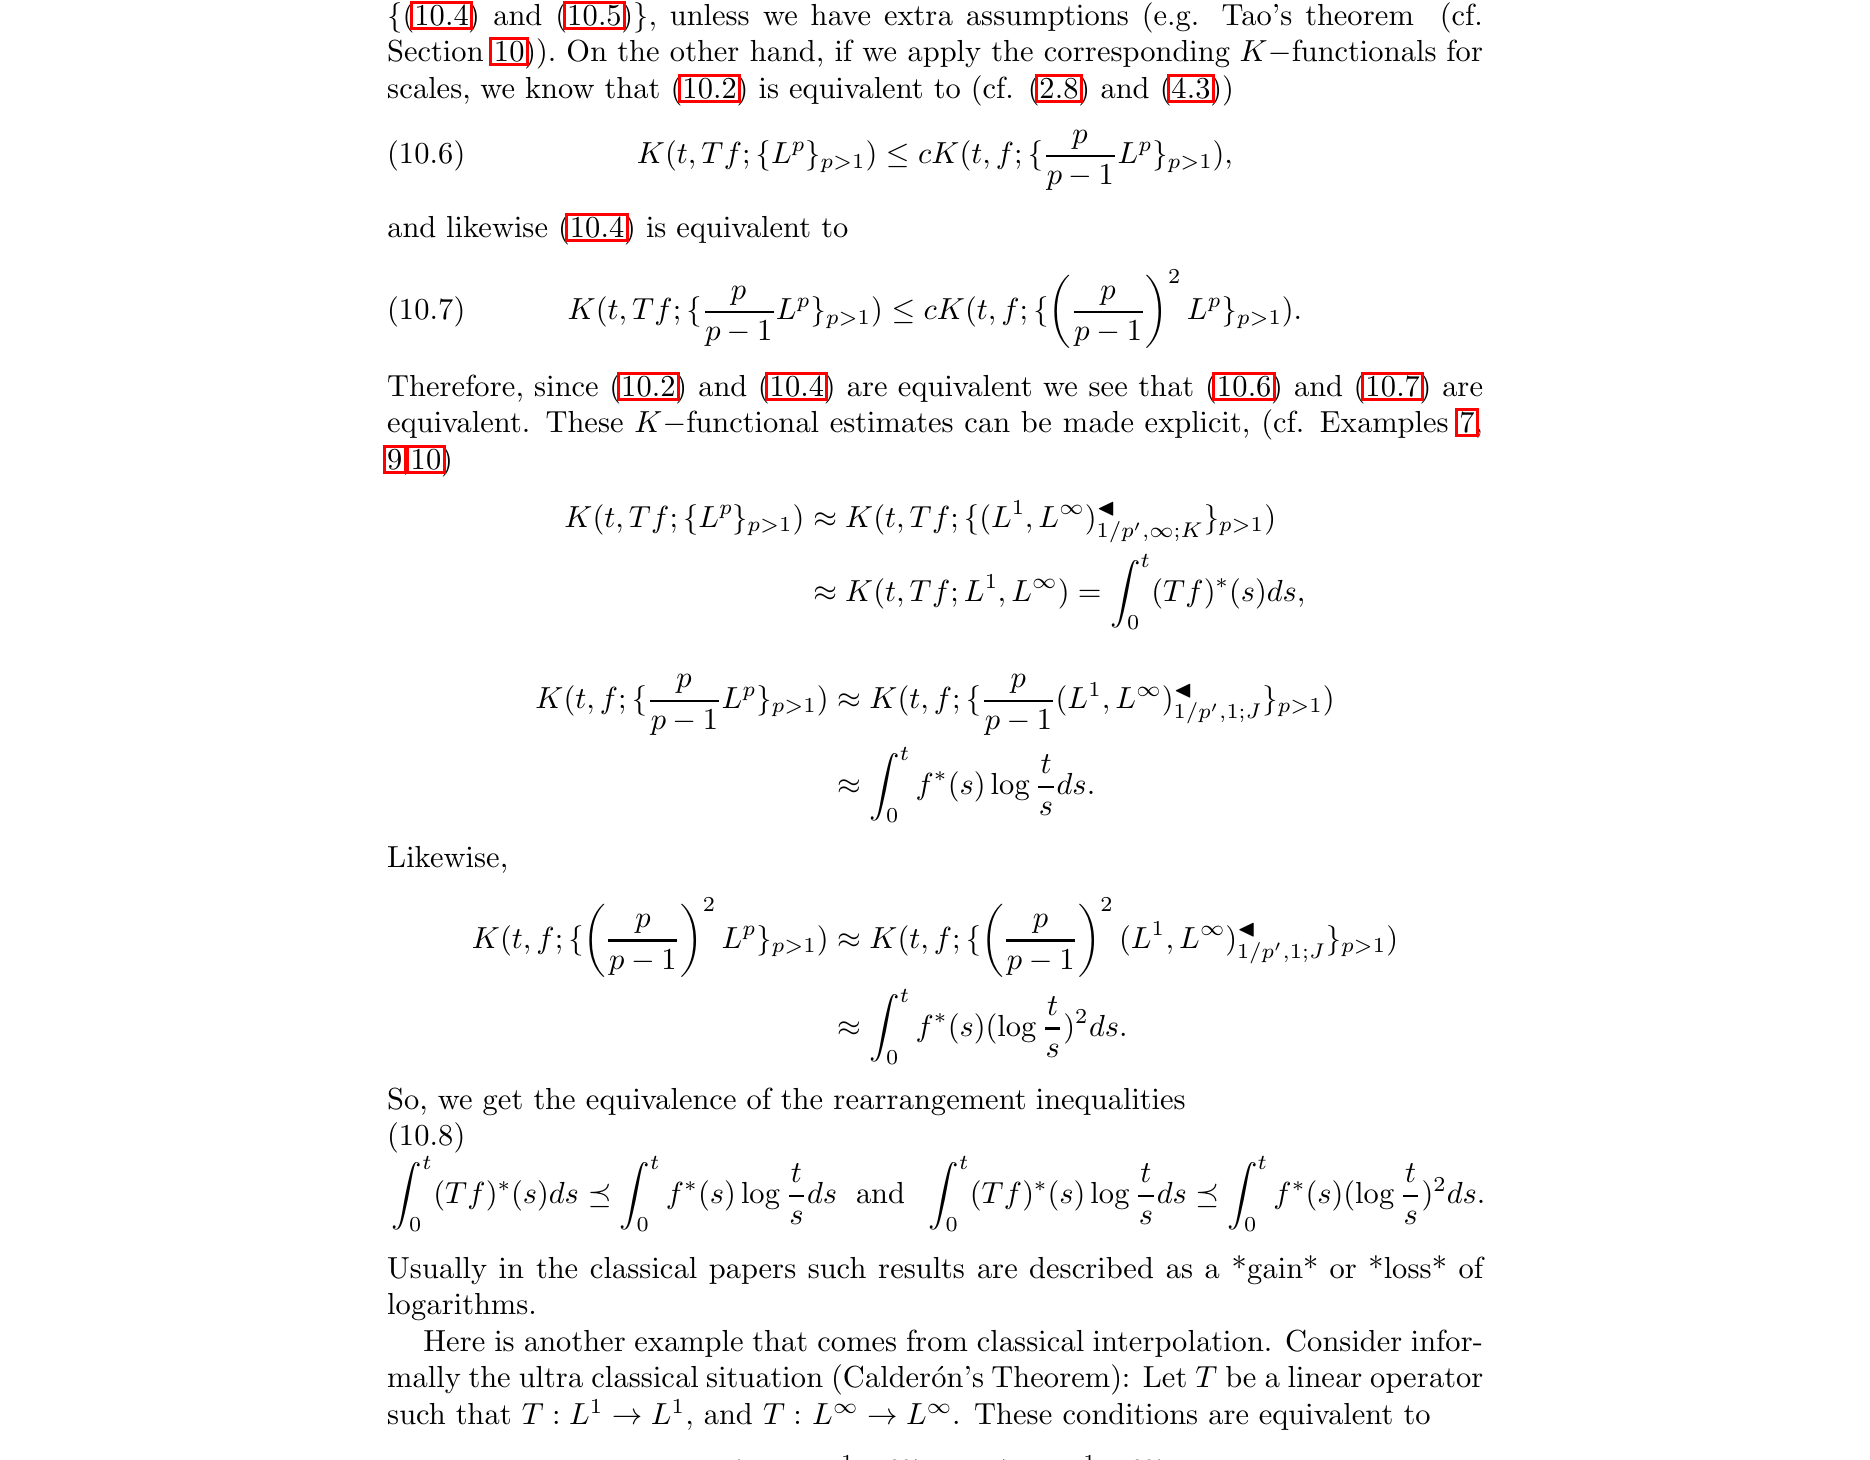
\includegraphics[width=\textwidth]{figures/rearrangement_inequalities_10_8_crop.png}
\caption{The two inequalities (10.8) in the source paper, page 41.}
\end{figure}

\begin{figure}[ht]
\centering

\includegraphics[width=\textwidth]{figures/open_problem_crop.png}
\caption{Problem 28 in the source paper, page 42.}
\end{figure}

For a measurable function $g$ on $(0,1)$, let $g^*$ denote the decreasing
rearrangement of $|g|$.  Written with explicit constants, the two properties
of an operator $T$ are
\begin{align}
 \int_0^t (Tf)^*(s)\,ds
 &\leq C_1\int_0^t f^*(s)\log\frac ts\,ds,
 \tag{A}\label{eq:A}\\
 \int_0^t (Tf)^*(s)\log\frac ts\,ds
 &\leq C_2\int_0^t f^*(s)\left(\log\frac ts\right)^2\,ds,
 \tag{B}\label{eq:B}
\end{align}
for every $f\in L^\infty(0,1)$ and every $0<t\leq1$.  The symbol
$\preceq$ in the source means that the relevant constant is independent of
$f$ and $t$.

\section{Idea of the proof}

There is a genuine one-way relation: integrating \eqref{eq:A} once in the
scale variable adds one logarithm to each side, so \eqref{eq:B} follows.
The converse would have to remove a logarithm, and that operation is not
order-preserving.

The obstruction can be isolated with a rank-one operator.  Pair the input
against the exact weight appearing on the right of \eqref{eq:B}, namely
$h(s)=\log^2(1/s)$, and output the resulting scalar as a constant function.
The dilation monotonicity of $f^*$ then proves \eqref{eq:B} with constant one.
But indicators of increasingly short initial intervals make this functional
larger than the right side of \eqref{eq:A} by an unbounded logarithmic factor.

\section{Result}

\begin{theorem}\label{thm:main}
The two properties \eqref{eq:A} and \eqref{eq:B} are not equivalent as
standalone operator inequalities.
\begin{enumerate}
\item For every operator $T$ for which the expressions are defined,
      \eqref{eq:A} with constant $C_1$ implies \eqref{eq:B} with constant
      $C_1/2$.
\item There is a rank-one linear operator $T$, bounded on $L^p(0,1)$ for
      every $1<p<\infty$, which satisfies \eqref{eq:B} with $C_2=1$ but
      satisfies \eqref{eq:A} for no finite constant $C_1$.
\end{enumerate}
In particular, the literal equivalence requested in Problem 28 of
\cite{AM} is false.
\end{theorem}

\section{Proof}

\subsection{The valid implication}

Assume \eqref{eq:A}.  Integrate it with respect to $du/u$ over $0<u<t$.
All integrands are nonnegative, so Tonelli's theorem gives
\begin{align*}
 \int_0^t \frac1u\int_0^u (Tf)^*(s)\,ds\,du
 &=\int_0^t (Tf)^*(s)\log\frac ts\,ds,\\
 \int_0^t \frac1u\int_0^u f^*(s)\log\frac us\,ds\,du
 &=\int_0^t f^*(s)\int_s^t\log\frac us\,\frac{du}{u}\,ds\\
 &=\frac12\int_0^t f^*(s)\left(\log\frac ts\right)^2\,ds.
\end{align*}
This proves \eqref{eq:B} with $C_2=C_1/2$.

\subsection{Construction and boundedness}

Put
\[
 h(s)=\left(\log\frac1s\right)^2,\qquad
 \ell(f)=\int_0^1 f(s)h(s)\,ds,
 \qquad Tf=\ell(f)\one.
\]
This is a rank-one linear operator.  If $1<p<\infty$ and
$q=p'=p/(p-1)$, then
\[
 \int_0^1 h(s)^q\,ds
 =\int_0^\infty x^{2q}e^{-x}\,dx
 =\Gamma(2q+1)<\infty.
\]
Consequently H\"older's inequality yields
\[
 \|Tf\|_p=|\ell(f)|\leq \|h\|_q\|f\|_p.
\]
Thus $T$ is bounded on every $L^p(0,1)$ with $1<p<\infty$ (and it is also
bounded on $L^\infty$).

We shall use the elementary rearrangement estimate
\[
 |\ell(f)|\leq\int_0^1 f^*(s)h(s)\,ds.
\]
For completeness, $h$ is nonnegative and decreasing.  For every measurable
$E\subset(0,1)$ of measure $m$, layer cake gives
$\int_Eh\leq\int_0^m h$.  Applying this inequality to the superlevel sets of
$|f|$ and integrating over the level proves
$\int|f|h\leq\int f^*h$, which proves the estimate.

\subsection{The second inequality holds}

Because $Tf$ is constant, $(Tf)^*(s)=|\ell(f)|$ on $(0,1)$.  Therefore
\[
 \int_0^t (Tf)^*(s)\log\frac ts\,ds
 =t|\ell(f)|.
\]
On the other hand, substitute $s=tu$ and use that $f^*$ is decreasing.  Since
$0<t\leq1$ implies $tu\leq u$,
\begin{align*}
 \int_0^t f^*(s)\left(\log\frac ts\right)^2\,ds
 &=t\int_0^1 f^*(tu)\left(\log\frac1u\right)^2\,du\\
 &\geq t\int_0^1 f^*(u)h(u)\,du\\
 &\geq t|\ell(f)|.
\end{align*}
Together with the preceding identity, this proves \eqref{eq:B} with $C_2=1$ for
every bounded $f$ and every $0<t\leq1$.

\subsection{The first inequality fails}

Let $0<\varepsilon<1$, set
$f_\varepsilon=\one_{(0,\varepsilon)}$, and write
$L=\log(1/\varepsilon)$.  Direct integration gives
\begin{align*}
 \ell(f_\varepsilon)
 &=\int_0^\varepsilon\left(\log\frac1s\right)^2\,ds
 =\varepsilon(L^2+2L+2),\\
 \int_0^1 f_\varepsilon^*(s)\log\frac1s\,ds
 &=\int_0^\varepsilon\log\frac1s\,ds
 =\varepsilon(L+1).
\end{align*}
At the permitted endpoint $t=1$, the quotient of the left side of
\eqref{eq:A} by its right side without $C_1$ is therefore
\[
 \frac{\varepsilon(L^2+2L+2)}{\varepsilon(L+1)}
 =L+1+\frac1{L+1}\longrightarrow\infty
 \qquad(\varepsilon\downarrow0).
\]
No finite $C_1$ can make \eqref{eq:A} hold.  This completes the proof of
Theorem~\ref{thm:main}.

\section{Verification and scope}\label{sec:scope}

The construction satisfies the explicit regularity present near the source
problem: it is one fixed linear operator, it is bounded on every
$L^p(0,1)$, $1<p<\infty$, and all test functions used above belong to
$L^1\cap L^\infty$.  The endpoint $t=1$ is included in the source range.

There is nevertheless an important interpretive distinction.  The discussion
preceding (10.8) begins with the stronger scale estimate
\[
 \|T\|_{L^p\to L^p}\lesssim \frac{p}{p-1}.
\]
If Problem 28 silently retains this as an additional hypothesis, then the
example above is outside that narrower class.  Indeed, the exact norm of the
rank-one operator is
\[
 \|T\|_{L^p\to L^p}=\|h\|_{p'}
 =\Gamma(2p'+1)^{1/p'}\asymp (p')^2
 \qquad(p\downarrow1),
\]
by Stirling's formula.  Thus the packet establishes a complete negative
answer to the literal standalone equivalence of the displayed inequalities;
it does not refute an explicitly augmented formulation with the
$O(p')$ norm-growth assumption already imposed.

\section{Novelty check and limitations}

The run indexes contained no matching result or attempt for arXiv:2004.03655,
Problem 28, logarithmic rearrangement inequalities, or rank-one
counterexamples.  Bounded web/arXiv searches on 9 August 2026 using the exact
problem phrase, close variants, the source authors, and later
Astashkin--Lykov--Milman work found no later answer or matching construction.
This is not an exhaustive novelty claim.  The result is noncomputational;
human review should focus on the intended scope of ``equivalence.''

{\small
\begin{thebibliography}{9}
\bibitem{AM}
S. Astashkin and M. Milman,
\emph{Extrapolation: Stories and Problems},
arXiv:2004.03655 (2020); Pure Appl. Funct. Anal. 6 (2021), no. 3, 651--707.
\end{thebibliography}
}

\end{document}
